\documentclass[12pt]{article}

% layout
\usepackage[top=0.5in, bottom=0.75in, left=0.625in, right=0.625in]{geometry}
\usepackage{multicol}
\usepackage{indentfirst}

% fonts and language support
\usepackage[utf8]{inputenc}
\usepackage[T2A]{fontenc}
\usepackage[english,russian]{babel}

% math and stuff
\usepackage{mathtools}              % Тот же amsmath, только с некоторыми поправками
\usepackage{amssymb}                % Математические символы
\usepackage{amsthm}                 % Оформление теорем
\usepackage{amstext}                % Текстовые вставки в формулы
\usepackage{amsfonts}               % Математические шрифты
\usepackage{icomma}                 % "Умная" запятая: $0,2$ --- число, $0, 2$ --- перечисление
\usepackage{enumitem}               % Для выравнивания itemize (\begin{itemize}[align=left])
\usepackage{array}                  % Таблицы и матрицы
\usepackage{multirow}
\usepackage{textcomp}
\usepackage{gensymb}
\usepackage{csvsimple}


% graphics
\usepackage{graphicx}
\usepackage{float}
\usepackage{subcaption}
\usepackage[export]{adjustbox}
\usepackage{wrapfig}
\usepackage[font=scriptsize]{caption}

% links and toc
\usepackage[colorlinks=true, urlcolor=blue, citecolor=black, linkcolor=blue]{hyperref}
\usepackage{biblatex}
\addbibresource{liter.bib}

% fonts settings
\linespread{1.5}

\begin{document}

\begin{titlepage}
  \center
  Федеральное государственное автономное образовательное учреждение\\
  высшего образования \\[.2cm]
  \textbf{\large <<Национальный исследовательский университет\\
    <<Высшая школа экономики>>}\\[.2cm]
  Факультет компьютерных наук\\[.2cm]
  \textbf{01.03.02}\ \  ОП <<Прикладная математика и информатика>>\\[4cm]
  \textbf{\LARGE Отчёт о прохождении практики}\\[2cm]
  {\flushleft
  \textbf{Студент}: Рубачёв Иван Викторович \\
  \textbf{Группа}: БПМИ161 \\
  \textbf{Вид практики}: Учебная\\[5.7cm]}

  \begin{multicols}{3}
    {\flushleft \scriptsize Руководитель:\vfill\columnbreak}
    {\flushleft \scriptsize Научный Сотрудник, Ст. Преп., \\[0.1em]}
    {\flushleft \scriptsize Лобачева Екатерина Максимовна}
    {\vskip5mm\rule{5cm}{0.15mm}}
  \end{multicols}
  \begin{multicols}{3}
    {\flushleft \scriptsize Куратор:\vfill\columnbreak}
    {\flushleft \scriptsize Младший Научный Сотрудник, \\}
    {\flushleft \scriptsize Чиркова Надежда Александровна}
    {\vskip5mm\rule{5cm}{0.15mm}}
  \end{multicols}
  Москва, 2018
\end{titlepage}

{
\hypersetup{linkcolor=black}
\tableofcontents
}

\newpage

\section*{Введение}
\addcontentsline{toc}{section}{\protect\numberline{}Введение}%
Большая часть успехов в распознавании речи, анализе текстов и изображений отчасти достигнута благодаря
увеличению объемов данных и усложнению моделей (рекуррентных нейросетей в частности). При таком подходе
возникают проблемы связанные с использованием полученных моделей с большим числом параметров в условиях ограничения ресурсов
(например, на мобильных устройствах). Прунинг -- один из методов решения данной проблемы.

Целью данной практики было изучение статьи \cite{DBLP:journals/corr/NarangDSE17} на тему прунинга рекуррентных 
нейронных сетей и дальнейшая реализация метода, описанного в ней алгоритма.
Перед началом работы над темой практики необходимо было изучить основы рекуррентных нейронных
сетей, выполнив лабораторную работу. Более детальная информация о 
методе прунинга из статьи, реализации базовой модели, реализации прунинга и результатах представлена 
в основной части отчета. 
\section*{Основная часть}
\addcontentsline{toc}{section}{\protect\numberline{}Основная часть}%

\subsection*{Обзор статьи <<Exploring Sparsity in Recurrent Neural Networks>> \cite{DBLP:journals/corr/NarangDSE17}}
\addcontentsline{toc}{subsection}{\protect\numberline{}Обзор статьи}%
Существуют различные подходы к прунингу нейронных сетей (Optimal Brain Damage \cite{Cun:1990:OBD:109230.109298},
Optimal Brain Surgeon \cite{Hassibi}, прунинг весов ниже порогового значения \cite{DBLP:journals/corr/HanPTD15}).

Авторы статьи, выбранной для изучения в рамках данной практики предлагают алгоритм прунинга рекуррентных нейроннных сетей.
Преимущества предлагаемого метода:
\begin{itemize}
  \item Вычислительная простота
  \item Отсутствие необходимости в дообучении модели
\end{itemize}
Метод заключается в обращении в $0$ весов, абсолютное значение которых ниже $\varepsilon$. Пороговое значение монотонно 
увеличивается в соответствии со следующими формулами:
\begin{equation}
  \varepsilon = \begin{cases}
    \theta \cdot \mathtt{diff} / \mathtt{freq}, & \mathtt{current\_itr} < \mathtt{ramp\_itr} \\
    \left(\theta \cdot \mathtt{diff} + \phi \cdot (\mathtt{current{\_}itr} - \mathtt{ramp\_itr} + 1)\right) / \mathtt{freq}, & \mathtt{current\_itr} \geqslant \mathtt{ramp\_itr}
  \end{cases}
  \label{eq:eps}
\end{equation}
Где $\mathtt{diff} = \mathtt{ramp\_itr} - \mathtt{start\_itr} + 1$, а \texttt{start\_itr}, \texttt{ramp\_itr}, \texttt{end\_itr} -- 
итерациии начала прунинга, увеличения скорости прунинга и конца прунинга соответственно. \texttt{current\_itr} -- текущая итерация, \texttt{freq} -- частота прунинга, $\phi$ и $\theta$ --
коэффициенты, определяющие интенсивность удаления весов. 

\newpage
$\theta$ определяется по формуле:

\begin{equation}
  \theta = \frac{2 \cdot q \cdot \mathtt{freq}}{2 \cdot (\mathtt{ramp\_itr} - \mathtt{start\_itr}) + 3 \cdot (\mathtt{end\_itr} - \mathtt{ramp\_itr})}
\end{equation}


Параметры \texttt{freq}, \texttt{ramp\_itr}, \texttt{start\_itr}, \texttt{end\_itr} и $\phi$ подбираются отдельно для каждого слоя сети. Параметр $q$ -- девяностый
перцентиль абсолютных значений весов обученной без применения прунинга модели. Алгоритм прунинга раз в \texttt{freq} итераций убирает из модели
веса, абсолютное значение которых меньше $\varepsilon$, и добавляет веса, значения которых больше $\varepsilon$ (Вес может стать больше порогового значения при 
обновлении весов в шаге градиентного спуска, т.к. градиенты для данных весов на этом шаге не изменяются). Таким образом удаление весов в данном алгоритме мягкое -- веса могут
вернуться в модель

\subsection*{Описание модели анализа тональности текста}
\addcontentsline{toc}{subsection}{\protect\numberline{}Описание модели}%

\subsubsection*{Данные и их предобработка}
В качестве набора данных для экспериментов был выбран датасет IMDB с рецензиями на фильмы \cite{maas-EtAl:2011:ACL-HLT2011}. В датасете собраны положительные
и отрицательные отзывы (по эмоциональной окраске). Размеры тренировочной и тестовой выборок $25000$ пар. Целевая переменная -- два класса 
($0$ -- негативная рецензия, $1$ -- положительная рецензия). На начальной стадии проекта для обработки данных использовался
модуль \texttt{torchtext}, затем он был заменен решением, написанным самостоятельно. Вся предобработка производится в модуле \texttt{utils}. Процесс можно описать пошагово:
\begin{itemize}
  \item
  Загрузка текстов. Все тексты и значения целевой переменной сохраняются в python массивах. В случае первой загрузки данных
  сохраняются как тестовые, так и тренировочные данные.
  \item
    Токенизация. На данном этапе из текстов удаляются или заменяются редко встречающиеся служебные символы (например \texttt{<br />} заменяется на \texttt{"\textbackslash n"}).
    Слова написанные в верхнем регистре заменяются на слова в нижнем регистре, при этом перед такими словами добавляется дополнительный токен \texttt{t\_up}. Также перед повторяющимися
    символами и словами добавлены специальные токены (с указанием числа повторов). После этого применяется токенизатор из модуля \texttt{spacy}. Этот этап обработки производится в параллельном 
    режиме (поэтому работает быстрее, чем \texttt{torchtext})
  \item Нумерализация. Далее, полученным на предыдущем шаге токенам присваиваются номеара. При этом остаются только
  $60000$ наиболее популярных токенов, из которых также отсеиваются те, которые встречаются реже $3$ раз. Полученные данные сохраняются на диск.
\end{itemize}
Помимо предобработки также написан нестандартный сэмплер (\texttt{torch.utils.data.Sampler}), который сортирует тексты в данных таким образом, что в батч попадают тексты
приблизительно одной длины. Независимо сортируются срезы размера ($\mathtt{batchSize} \times 50$), затем сортируются срезы размера \texttt{batchSize}.

При обучении тексты в батче дополняются слева специальным символом (единица после нумерализации) до длины максимального из них.
\subsubsection*{Архитектура модели}
Базовая модель представляет собой однослойную рекуррентную нейронную сеть с архитектурой long-short term memory (LSTM) \cite{Hochreiter:1997:LSM:1246443.1246450}, на вход которой подаются векторные представления
токенов (word embedding), на выходе находится один линейный слой. Для регуляризации используется рекуррентный дропаут \cite{1512.05287} с вероятностью $p=0.65$ (одна и та же маска применяется на каждом шаге RNN) после word embedding,
обычный дропаут \cite{JMLR:v15:srivastava14a} с вероятностью $p=0.5$ на входе линейного слоя, также используется дропаут в word embedding \cite{1512.05287} (зануляются векторы для отдельных слов с вероятностью $p=0.1$).

Все дальнейшие эксперименты производились с моделью со следующими параметрами:
\begin{center}
  \begin{tabular}{ c  c  c }
    \hline
    Layer & Input dim & Output dim \\ \hline
    Word Embedding & 60002 & 300 \\
    LSTM & 300 & 128 \\
    Linear Layer & 128 & 1 \\ \hline
  \end{tabular}
\end{center}

Общее число параметров в модели: $18,220,889$.

\newpage

\subsubsection*{Результаты}
После обучения $8$ эпох, были получены следующие результаты:

\begin{center}
\begin{tabular}{cccccc}
  \hline
  Epoch & Time (s) & Train Loss & Test Loss & Train Acc & Test Acc \\ \hline
  1 & 108.65 & 35.958 & 27.779 & 0.68 & 0.78 \\
  2 & 111.31 & 24.467 & 24.578 & 0.84 & 0.84 \\
  3 & 98.24 & 19.873 & 20.623 & 0.87 & 0.87 \\
  4 & 109.19 & 17.795 & 22.941 & 0.89 & 0.87 \\
  5 & 106.14 & 16.155 & 20.806 & 0.9 & 0.87 \\
  6 & 105.55 & 14.864 & 21.017 & 0.91 & 0.87 \\
  7 & 103.66 & 13.645 & 22.307 & 0.92 & 0.87 \\
  8 & 104.53 & 11.989 & 21.826 & 0.93 & 0.86 \\ \hline
\end{tabular}
\end{center}

Здесь точность -- доля правильо классифицированных текстов, а функция потерь -- бинарная перекрестная энтропия 
($\ell(x, y) = \sum l_n, \quad l_n = - w_n \left[ t_n \cdot \log \sigma(x_n) + (1 - t_n) \cdot \log (1 - \sigma(x_n)) \right]$). 
Полученные качество соотвестствует модели такого типа из работы \cite{stanfordrep}.

\subsection*{Реализация метода прунинга}
\addcontentsline{toc}{subsection}{\protect\numberline{}Реализация метода прунинга}%
\subsubsection*{Описание алгортма}
Данный метод заключается в поддержании набора масок для весов модели. Изначально 
маски инициализируются единицами. После каждого шага оптимизации веса перемножаются 
с масками, таким образом $1$ в маске означает, что соответствующий вес используется в модели, а $0$ -- вес не используется. Также с регулярным интервалом маски обновляются, выставлением в $0$/$1$ элементов,
соответствующих весам, абсолютное значение которых меньше/больше порогового значения, подсчитанного 
по формуле \ref{eq:eps}.
\subsubsection*{Реализация в pytorch}
Вспомогательные классы, добавляющие поддержку прунинга находятся в модуле
\texttt{pruner.py}. Класс \texttt{ModelPruner} инициализирует для каждого 
параметра модели класс \texttt{WeightPruner}, который затем обновляет и применяет
маску к своему параметру в соотвестствии с параметрами, которые указаны в 
конфигурационном файле. Маски применялись ко всем параметрам модели (в том числе матрице слоя 
представлений и линейному слою), кроме сдвигов (bias).

\subsubsection*{Результаты}
При применении прунинга, были получены следующие результаты:

\begin{center}
\begin{tabular}{ccccccc}
  \hline
  Epoch & Time (s) & Train Loss & Test Loss & Train Acc & Test Acc & Sparsity\\
  \hline
  1 & 110.37 & 35.547 & 25.801 & 0.69 & 0.83 & 0.0\\
  2 & 100.53 & 24.139 & 23.167 & 0.84 & 0.81 & 0.08\\
  3 & 103.67 & 19.789 & 22.054 & 0.87 & 0.84 & 0.26\\
  4 & 101.6 & 16.809 & 20.582 & 0.89 & 0.87 & 0.45\\
  5 & 103.79 & 15.053 & 20.901 & 0.91 & 0.87 & 0.64\\
  6 & 107.55 & 14.253 & 21.799 & 0.91 & 0.87 & 0.81\\
  7 & 112.47 & 14.276 & 24.024 & 0.92 & 0.87 & 0.94\\
  8 & 104.8 & 11.653 & 22.526 & 0.93 & 0.84 & 0.94\\
  9 & 100.44 & 11.072 & 24.969 & 0.93 & 0.86 & 0.94\\
  10 & 113.35 & 11.093 & 22.774 & 0.93 & 0.85 & 0.94\\
  \hline
\end{tabular}
\end{center}

В данном случае применение прунинга не ухудшило качество на тестовой выборке (Если взять модель после $7$ эпохи).

Ниже приведены графики числа удаленных весов для различных параметров модели:

\begin{center}
  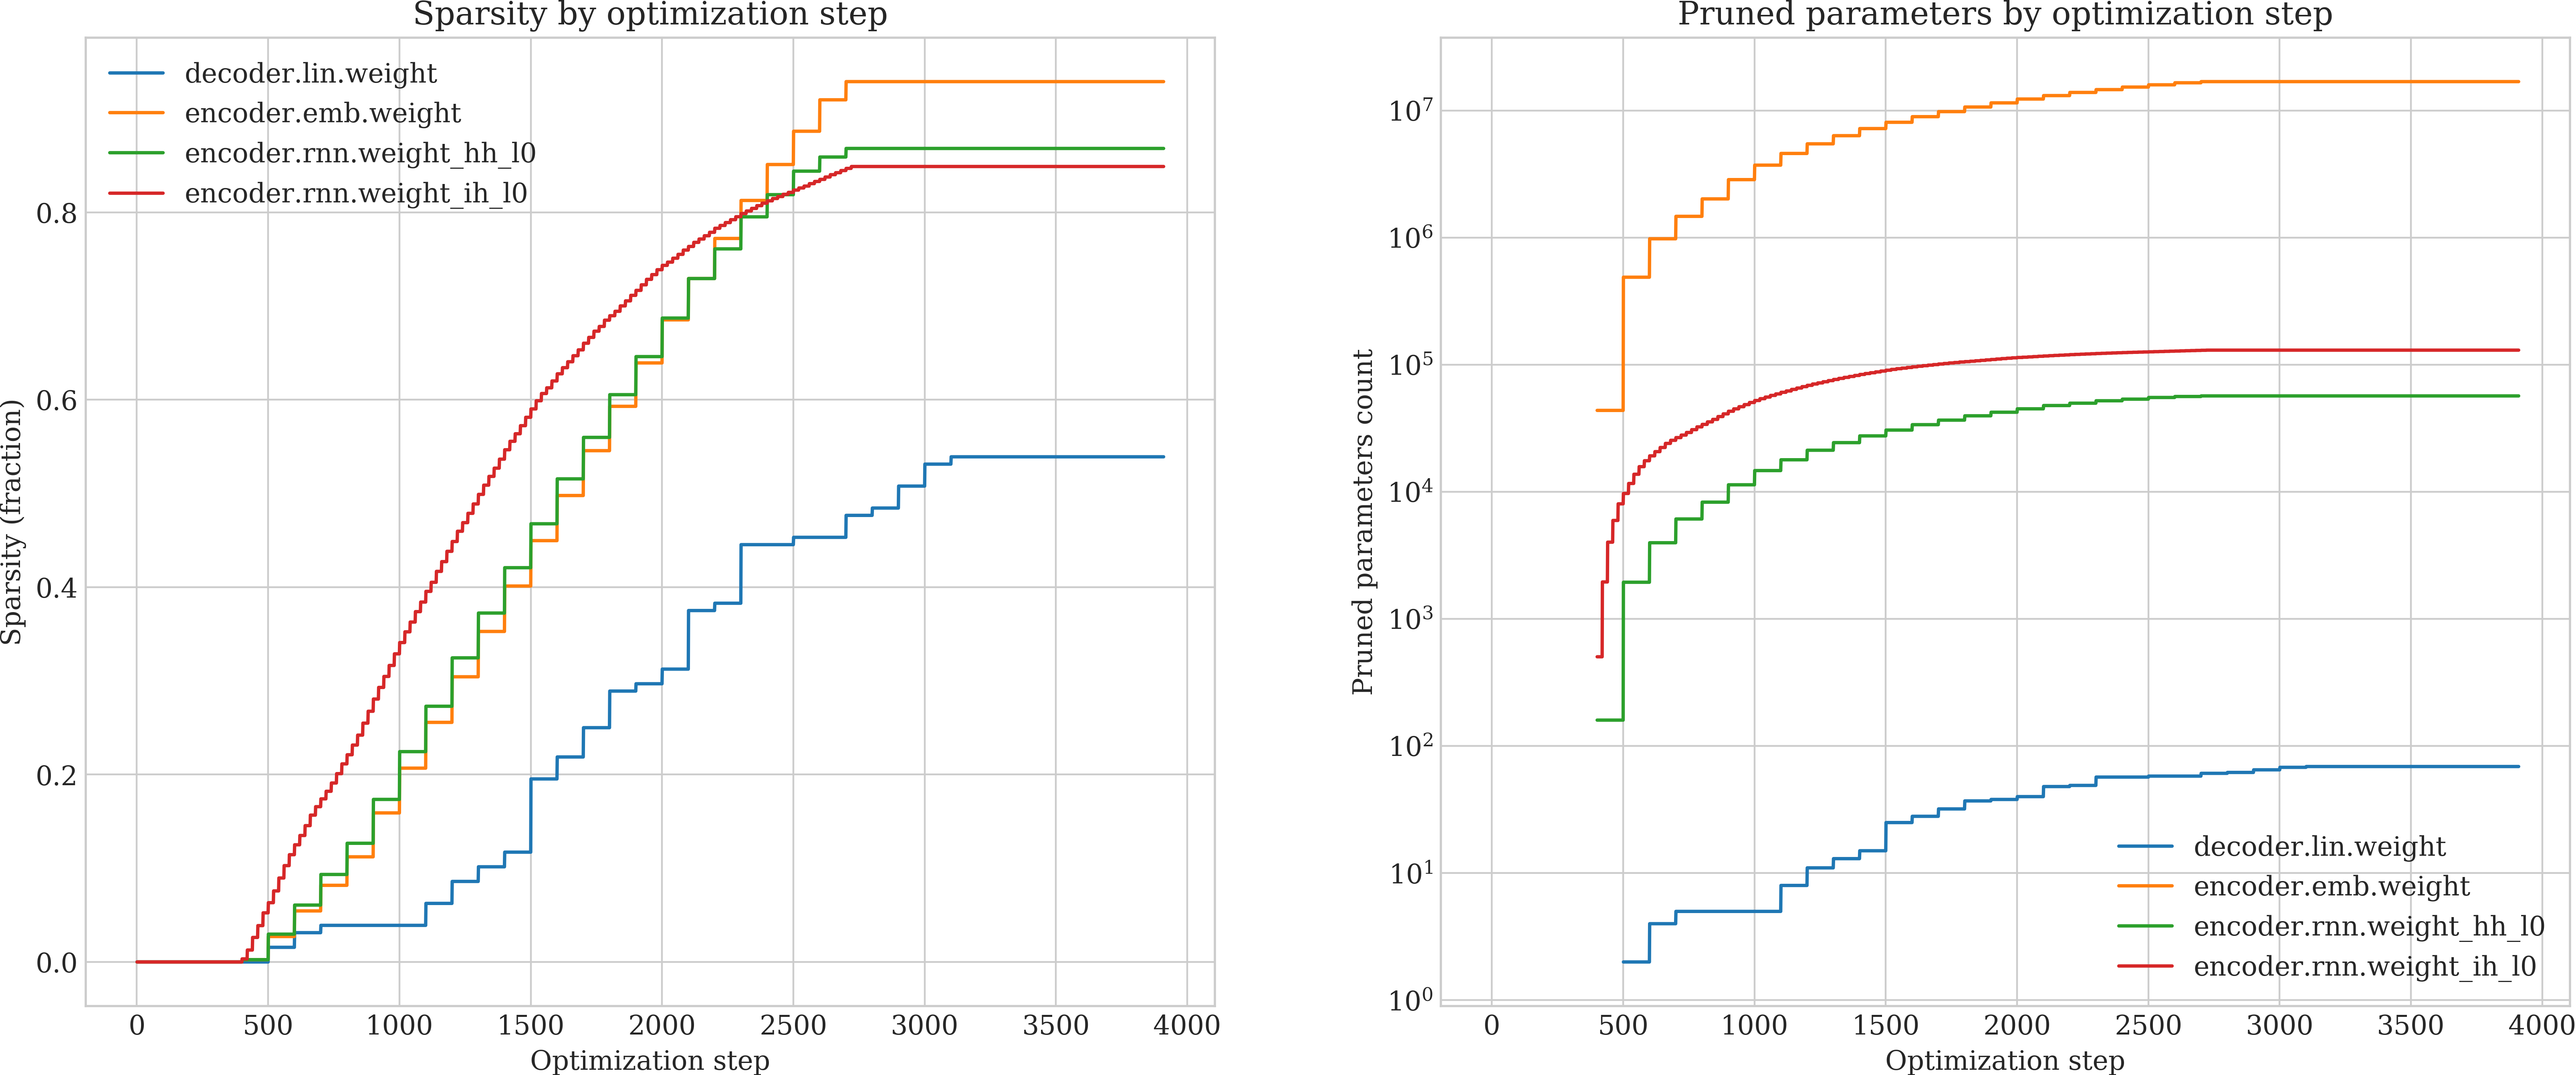
\includegraphics[width=0.96\textwidth]{results}
\end{center}

Графики построены для модели с конфигурацией описанной в файле \href{https://github.com/puhsu/pruning/blob/master/configs/base.yaml}{base.yaml}. Слева изображена зависимость разреженности весов от итерации обучения для различных параметров модели при прунинге.
На графике справа изображена зависимость числа удаленных параметров от итерации обучения.

\section*{Заключение}
\addcontentsline{toc}{section}{\protect\numberline{}Заключение}%
В результате выполнения практики, был реализован и протестирован алгоритм прунинга рекуррентных нейроннных сетей. 
Код с инструкциями к запуску выложен в открытый доступ: \url{https://github.com/puhsu/pruning}
Данная практика оказалась очень полезной с образовательной точки зрения. В процессе 
решения задачи были изучены основные принципы работы рекуррентных нейронных сетей (а также 
работы с текстовыми данными), библиотека \texttt{pytorch}, методы 
<<сжатия>> нейронных сетей. Также во время выполнения задания были изучены много источников 
(статей, opensource проектов, видеолекций). Например, во время изучения основ RNN были найдены 
блоги \cite{colah, karpathy}, при реализации модели были использованы
идеи из статьи \cite{DBLP:journals/corr/abs-1801-06146}. К сожалению, далеко 
не все идеи были опробованы. В качестве следующих шагов по данному проекту было бы интересно
провести следующие эксперименты: удалять веса из языковой модели во время 
обучения на тех же данных (не исключая рецензий без целевой переменной), и затем дообучить полученную
модель для задачи классификации. Также стоит попробовать использовать библиотеку \cite{neta_zmora_2018_1297430}, в которой 
есть реализации различных алгоритмов прунинга.

\newpage

\nocite{*}
\printbibliography[title={Список используемых источников}]
\addcontentsline{toc}{section}{\protect\numberline{}Список используемых источников}


\end{document}
